% !TEX program = xelatex
\documentclass[12pt,a4paper,fontset=fandol]{ctexart}
\usepackage[left=22mm,right=22mm,top=22mm,bottom=22mm]{geometry}
\usepackage{amsmath,amssymb,bm,mathtools}
\usepackage{graphicx,xcolor,booktabs,longtable,array,calc}
\usepackage{tikz}
\usetikzlibrary{arrows.meta,calc,decorations.pathmorphing}
\usepackage{setspace,enumitem,fancyhdr}
\usepackage[unicode,hidelinks]{hyperref}
\setstretch{1.24}
\setlength{\parindent}{2em}
\setlength{\parskip}{.35em}
\setlength{\emergencystretch}{2em}
\setlist{nosep,leftmargin=2em}
\setcounter{secnumdepth}{-1}
\ctexset{section={format=\Large\bfseries,beforeskip=1em,afterskip=.7em},
subsection={format=\large\bfseries,beforeskip=.8em,afterskip=.4em},
subsubsection={format=\normalsize\bfseries,beforeskip=.7em,afterskip=.3em}}
\allowdisplaybreaks[2]
\tikzset{arr/.style={-{Stealth[length=2mm]},semithick},
dot/.style={circle,fill,inner sep=1.5pt}}
\providecommand{\tightlist}{\setlength{\itemsep}{0pt}\setlength{\parskip}{0pt}}
\providecommand{\pandocbounded}[1]{#1}
\newsavebox{\diagrambox}
\pagestyle{fancy}
\fancyhf{}
\renewcommand{\headrulewidth}{0pt}
\fancyfoot[C]{\small \thepage}
\setlength{\headheight}{16pt}
\begin{document}
\begin{titlepage}
\thispagestyle{empty}
\vspace*{27mm}
\begin{center}
{\LARGE\bfseries 第40届全国中学生物理竞赛\par}
\vspace{8mm}
{\LARGE\bfseries 复赛理论试题\par}
\vspace{17mm}
{\Large 试题版\par}
\end{center}
\vfill
\end{titlepage}
\setcounter{page}{1}
本卷共8题，总分320分。考试时间：9:00-12:00。所有需要评阅的解答均须写在答题纸上。

\section{第 1
题　手机镜头的等效焦距与主点（40分）}\label{ux7b2c-1-ux9898-ux624bux673aux955cux5934ux7684ux7b49ux6548ux7126ux8dddux4e0eux4e3bux70b940ux5206}

手机镜头由多个光学元件组成，图像传感器能记录物体的像，借助软件可读出像的实际尺寸。将镜头视为结构固定的共轴理想透镜组，可把物像关系等效为一个凸透镜，使用薄透镜成像公式计算。但物距、像距与焦距的起点分别为光轴上的物方主点
\(H\) 和像方主点
\(H'\)，这些主点不必与某个透镜的光心重合。本题所有光路均满足近轴条件。

\begin{center}
\begin{minipage}{\linewidth}
\centering\begingroup\sbox{\diagrambox}{\small
\begin{tikzpicture}[scale=.9]
\draw[arr] (-.6,0)--(7.8,0);
\draw[dashed] (2,-1)--(4.8,-1)--(4.8,1)--(2,1)--cycle;
\draw[densely dashed] (2.7,-.75)--(2.7,.75) node[above] {$H$};
\draw[densely dashed] (4.1,-.75)--(4.1,.75) node[above] {$H'$};
\fill (0,0) circle(2pt) node[above] {物};
\fill (7,0) circle(2pt) node[above] {像};
\draw[<->] (0,-.55)--(2.7,-.55) node[midway,below] {$u$};
\draw[<->] (4.1,-.55)--(7,-.55) node[midway,below] {$v$};
\node at (3.4,-1.45) {透镜组：距离分别从两主点起算};
\end{tikzpicture}
}
\ifdim\wd\diagrambox>.88\linewidth
\sbox{\diagrambox}{\resizebox{.88\linewidth}{!}{\usebox{\diagrambox}}}\fi
\ifdim\ht\diagrambox>.38\textheight
\resizebox{!}{.38\textheight}{\usebox{\diagrambox}}
\else\usebox{\diagrambox}\fi
\par\smallskip{\small 透镜组的两主点与薄透镜的单光心\par}\endgroup\end{minipage}\end{center}

（1）主点封装在镜头内部，位置未知，无法直接测量物距。沿光轴移动一段与光轴垂直、长为
\(l\) 的刻度尺，在物距 \(u_1,u_2\) 处分别成像，测得移动距离
\(s=u_2-u_1\) 和对应像长 \(l_1,l_2\)。求：（i）等效焦距
\(F\)；（ii）物距 \(u_1\)。结果均用 \(l,l_1,l_2,s\) 表示。

（2）透镜组由焦距分别为 \(f_1,f_2\) 的共轴薄透镜组成，光心为
\(O_1,O_2\)，间距 \(d\)。物经两透镜成像时，存在横向放大率为 \(+1\)
的一对物面和像面，称为主平面，其与光轴的交点为 \(H,H'\)。（i）将 \(H\)
看作透镜1的``物''，求它相对 \(O_1\) 的物距；将 \(H'\)
看作透镜2的``像''，求它相对 \(O_2\) 的像距。（ii）物方距离从 \(H\)
起算，像方距离从 \(H'\) 起算，求物方焦距 \(F\) 和像方焦距 \(F'\)。

\clearpage

\section{第 2
题　半圆管活塞的临界稳定性（40分）}\label{ux7b2c-2-ux9898-ux534aux5706ux7ba1ux6d3bux585eux7684ux4e34ux754cux7a33ux5b9aux602740ux5206}

将粗细均匀、两端封闭的细玻璃管弯成半径为 \(r\)
的半圆环，竖直固定于水平地面，两端与地面接触。管的横截面尺寸远小于
\(r\)。管内有质量为 \(m\)
的薄活塞，与管壁密接，摩擦忽略；活塞相对竖直方向的角位置为
\(\theta\)。两侧各有 \(n\) 摩尔理想气体，其温度始终与外界温度 \(T\)
相同，所有气体状态变化均可视为准静态。重力加速度为 \(g\)，普适气体常量为
\(R\)。

\begin{center}
\begin{minipage}{\linewidth}
\centering\begingroup\sbox{\diagrambox}{\small
\begin{tikzpicture}[scale=1]
\draw[thick] (-3.4,0)--(3.4,0);
\draw[very thick] (3,0) arc(0:180:3);
\draw[dashed] (0,0)--(0,3);
\draw[dashed] (0,0)--(70:3);
\draw[thick] (70:2.82)--(70:3.18);
\draw[<->] (0,0)--(145:3) node[midway,above,fill=white,inner sep=1pt] {$r$};
\draw[arr] (0,1.0) arc(90:70:1);
\node at (.3,1.25) {$\theta$};
\node at (-1.45,2.1) {$n,\ T$};
\node at (1.8,1.25) {$n,\ T$};
\node[above right] at (70:3.2) {活塞 $m$};
\node at (-2.2,2.9) {$r(\pi/2+\theta)$};
\node at (3.3,2.3) {$r(\pi/2-\theta)$};
\end{tikzpicture}
}
\ifdim\wd\diagrambox>.88\linewidth
\sbox{\diagrambox}{\resizebox{.88\linewidth}{!}{\usebox{\diagrambox}}}\fi
\ifdim\ht\diagrambox>.38\textheight
\resizebox{!}{.38\textheight}{\usebox{\diagrambox}}
\else\usebox{\diagrambox}\fi
\par\smallskip{\small 半圆管、活塞与两侧气体长度\par}\endgroup\end{minipage}\end{center}

（1）当 \(T\) 高于某临界温度 \(T_c\) 时，\(\theta=0\) 为稳定平衡位置。求
\(T_c\) 及活塞在该位置附近微振动的圆频率。

（2）\(T=T_c\) 时，判断中央平衡位置的稳定性。

以下可视 \(T_c\) 为已知量，不必代入第（1）问结果。

（3）\(T<T_c\) 时，求稳定平衡角 \(\theta_0\) 满足的方程，并求 \(T\)
略低于 \(T_c\) 时 \(\theta_0\) 的最低非零阶近似。

（4）求 \(T<T_c\) 时稳定位置附近的微振动圆频率
\(\omega_0(\theta_0)\)，表达式可含 \(\theta_0\)，不可含 \(T\)；并给出
\(T\) 略高于及略低于 \(T_c\) 时圆频率随温度的变化。

（5）\(T<T_c\) 时，初始速度近似为零，求从正中央运动到可到达的角位置
\(\theta\) 时角速度的大小。

\clearpage

\section{第 3
题　可动楔块上的滚动与滑动（40分）}\label{ux7b2c-3-ux9898-ux53efux52a8ux6954ux5757ux4e0aux7684ux6edaux52a8ux4e0eux6ed1ux52a840ux5206}

倾角为 \(\theta\)、质量为 \(M\)
的三角形楔块放在光滑水平地面上，其斜面上有质量为 \(m\)、半径为 \(r\)
的均质圆球。圆球从静止开始向下运动，过程中楔块无转动。重力加速度为
\(g\)，球与楔块间的静摩擦系数和滑动摩擦系数均为 \(\mu\)。

\begin{center}
\begin{minipage}{\linewidth}
\centering\begingroup\sbox{\diagrambox}{\small
\begin{tikzpicture}[scale=1]
\draw[thick] (-.5,0)--(6.4,0);
\draw[thick,fill=gray!10] (0,0)--(5,0)--(5,2.6)--cycle;
\draw[thick] (3.58,2.4) circle(.48);
\fill (3.58,2.4) circle(1.5pt);
\node[above] at (3.58,2.95) {$m,\ r$};
\node at (3.8,.7) {$M$};
\draw (1,0) arc(0:27.47:1);
\node at (1.15,.28) {$\theta$};
\draw[arr] (2.4,1.6)--(1.2,.976) node[left] {$v_c$};
\draw[arr] (4.2,.45)--(5.6,.45) node[right] {$v_0$};
\node at (2.8,-.55) {球向左下运动，楔块向右};
\end{tikzpicture}
}
\ifdim\wd\diagrambox>.88\linewidth
\sbox{\diagrambox}{\resizebox{.88\linewidth}{!}{\usebox{\diagrambox}}}\fi
\ifdim\ht\diagrambox>.38\textheight
\resizebox{!}{.38\textheight}{\usebox{\diagrambox}}
\else\usebox{\diagrambox}\fi
\par\smallskip{\small 圆球与可动楔块，斜面向左下降\par}\endgroup\end{minipage}\end{center}

（1）若 \(\mu\) 足够大，圆球无滑动地滚下，求：（i）楔块对地加速度大小
\(a_0\)；（ii）球质心相对楔块的加速度大小
\(a_c\)；（iii）地面对楔块的支持力 \(N\)；（iv）楔块对球的支持力
\(N_1\)；（v）保持纯滚动所需的最小摩擦系数 \(\mu_0\)。

（2）若 \(\mu<\mu_0\) 且斜面足够长，求从静止开始经过 \(\Delta t\)
后，球与楔块接触点 \(P\) 相对楔块的速度。

\clearpage

\section{第 4
题　编木拱桥的几何、受力与摩擦（40分）}\label{ux7b2c-4-ux9898-ux7f16ux6728ux62f1ux6865ux7684ux51e0ux4f55ux53d7ux529bux4e0eux6469ux64e640ux5206}

《清明上河图》中的编木拱桥通过构件互相挤压、支持与摩擦保持结构。现考虑仅有三个单元、左右对称的简化侧视模型。在竖直平面内，将每对平行长杆等效为一根质量为
\(M\) 的杆，系统包含三根短杆 \(A,A',B\) 与三根长杆
\(C,D,D'\)。所有杆为半径 \(R\) 的圆柱，无槽口；短杆质量均为
\(m\)，长杆长度均为 \(L\)。长杆互不接触，短杆 \(B\)
表面光滑，其余杆间摩擦系数为 \(\mu\)，杆与地面静摩擦系数为
\(\mu'\)。\(D,D'\) 与地面夹角为 \(\theta\)，重力加速度为 \(g\)。

\begin{center}
\begin{minipage}{\linewidth}
\centering\begingroup\sbox{\diagrambox}{\small
\begin{tikzpicture}[scale=.75]
\draw[thick] (-.8,0)--(9.5,0);
\begin{scope}[rotate=45]
\draw[thick,fill=gray!12] (0,0)--(7.5,0)--(7.5,.414214)--(0,.414214)--cycle;
\end{scope}
\begin{scope}[shift={(8.778175,0)},rotate=135]
\draw[thick,fill=gray!12] (0,-.414214)--(7.5,-.414214)--(7.5,0)--(0,0)--cycle;
\end{scope}
\draw[thick,fill=white] (.639088,3.474874)--(8.139088,3.474874)--(8.139088,3.889088)--(.639088,3.889088)--cycle;
\draw[thick,fill=white] (2.389088,3.267767) circle(.207107);
\draw[thick,fill=white] (6.389088,3.267767) circle(.207107);
\draw[thick,fill=white] (4.389088,4.096194) circle(.207107);
\node[font=\scriptsize] at (2.389088,3.267767) {$A$};
\node[font=\scriptsize] at (6.389088,3.267767) {$A'$};
\node[font=\scriptsize] at (4.389088,4.096194) {$B$};
\node[left] at (.639088,3.681981) {$C$};
\node[left] at (.35,.65) {$D$};
\node[right] at (8.4,.65) {$D'$};
\draw (1,0) arc(0:45:1); \node at (1.12,.35) {$\theta$};
\draw[<->,dashed] (-.6,.6)--(2.228427,3.428427) node[midway,left] {$a$};
\draw[<->,dashed] (-1,1)--(3.242641,5.242641) node[midway,left] {$b$};
\node at (4.4,-.7) {侧视投影：相交长杆不发生接触};
\end{tikzpicture}
}
\ifdim\wd\diagrambox>.88\linewidth
\sbox{\diagrambox}{\resizebox{.88\linewidth}{!}{\usebox{\diagrambox}}}\fi
\ifdim\ht\diagrambox>.38\textheight
\resizebox{!}{.38\textheight}{\usebox{\diagrambox}}
\else\usebox{\diagrambox}\fi
\par\smallskip{\small 六杆简化模型，短杆以圆形截面表示\par}\endgroup\end{minipage}\end{center}

（1）\(D\) 杆下端到与 \(A\) 杆接触点的长度为 \(a\)，求下端到与 \(B\)
杆接触点的长度 \(b\)。

（2）利用左右对称，分析 \(A,B,C,D\) 的受力。短杆 \(A\) 的上方与 \(C\)
接触处有向下的 \(N_1\)、向右的 \(f_1\)；与斜杆 \(D\)
接触处有垂直斜面向左上的 \(N_2\)、沿斜面向右上的 \(f_2\)，并受向下重力
\(mg\)。短杆 \(B\) 受 \(C\) 向上的 \(N_3\)、两斜杆向下内侧的
\(N_4\)，以及重力 \(mg\)。画出 \(C,D\) 的受力图，对 \(A,B,C,D\)
分别列力平衡及必要的力矩平衡方程，每对作用力和反作用力用相同符号。

（3）\(M=6m\)，\(\theta=45^\circ\)，\(L=30\,\mathrm{cm}\)，\(a=16\,\mathrm{cm}\)，\(R=2(\sqrt2-1)\,\mathrm{cm}\)。求结构保持平衡时
\(\mu,\mu'\) 应满足的数值条件，保留三位有效数字。

\clearpage

\section{第 5
题　电偶极子场中的点电荷运动（40分）}\label{ux7b2c-5-ux9898-ux7535ux5076ux6781ux5b50ux573aux4e2dux7684ux70b9ux7535ux8377ux8fd0ux52a840ux5206}

质量为 \(m\)、电荷量为 \(e>0\) 的点电荷在固定于原点 \(O\)
的电偶极子作用下运动。偶极矩
\(\boldsymbol p=p\hat{\boldsymbol z}\)，点电荷位置为
\(\boldsymbol r(t)\)，其大小为 \(r(t)\)，与偶极矩夹角为
\(\theta(t)\)。初始位置满足
\(r(0)=r_0>0\)、\(\theta(0)=\theta_0\)。真空介电常量为
\(\varepsilon_0\)，场和电势为

\[\boldsymbol E=\frac{3(\boldsymbol p\cdot\hat{\boldsymbol r})\hat{\boldsymbol r}-\boldsymbol p}
{4\pi\varepsilon_0r^3},\qquad
\phi=\frac{\boldsymbol p\cdot\boldsymbol r}{4\pi\varepsilon_0r^3}.\]

\begin{center}
\begin{minipage}{\linewidth}
\centering\begingroup\sbox{\diagrambox}{\small
\begin{tikzpicture}[scale=1]
\draw[arr] (0,-1.2)--(0,3.4) node[above] {$z$};
\draw[arr,very thick] (0,-.6)--(0,.6) node[left] {$\boldsymbol p$};
\fill (0,0) circle(1.6pt) node[below right] {$O$};
\draw[arr] (0,0)--(2.4,2.1) node[midway,below right] {$\boldsymbol r$};
\fill (2.4,2.1) circle(2pt) node[right] {$e,\ m$};
\draw (0,1) arc(90:41.19:1);
\node at (.46,1.2) {$\theta$};
\draw[dashed] (2.4,2.1)--(0,2.1);
\end{tikzpicture}
}
\ifdim\wd\diagrambox>.88\linewidth
\sbox{\diagrambox}{\resizebox{.88\linewidth}{!}{\usebox{\diagrambox}}}\fi
\ifdim\ht\diagrambox>.38\textheight
\resizebox{!}{.38\textheight}{\usebox{\diagrambox}}
\else\usebox{\diagrambox}\fi
\par\smallskip{\small 位置矢量、偶极矩与夹角\par}\endgroup\end{minipage}\end{center}

（1）假定点电荷在垂直 \(z\) 轴的平面内绕 \(z\) 轴作匀速圆周运动，求
\(\theta_0\) 和速度 \(v_0\)。

（2）假定 \(t=0\) 时点电荷静止，求：（i）角动量大小 \(L\) 对 \(\theta\)
的关系；（ii）径向速率 \(v_r\) 对 \(r\) 的关系；（iii）运动有界的
\(\theta_0\) 条件，及取边界值时在竖直平面内的轨道；（iv）运动无界时
\(r(t)\)。不讨论点电荷与偶极子碰撞以后的情况。

\clearpage

\section{第 6
题　涡电流的悬浮与热效应（40分）}\label{ux7b2c-6-ux9898-ux6da1ux7535ux6d41ux7684ux60acux6d6eux4e0eux70edux6548ux5e9440ux5206}

交变磁场在导体内部产生涡电流，可用于加热、制动和悬浮。半径为 \(b\)
的水平圆线圈固定于桌面，电流为 \(I(t)=I_0\cos\omega t\)。重力大小为
\(G\)、半径为 \(a\)、电导率为 \(\sigma\)
的导体球位于线圈中心正上方，高度为 \(h\)。已知 \(a\ll b\)，趋肤深度

\[\delta=\sqrt{\frac2{\omega\mu_0\sigma}}\ll a,\]

其中 \(\mu_0\) 为真空磁导率，忽略电磁辐射。

\begin{center}
\begin{minipage}{\linewidth}
\centering\begingroup\sbox{\diagrambox}{\small
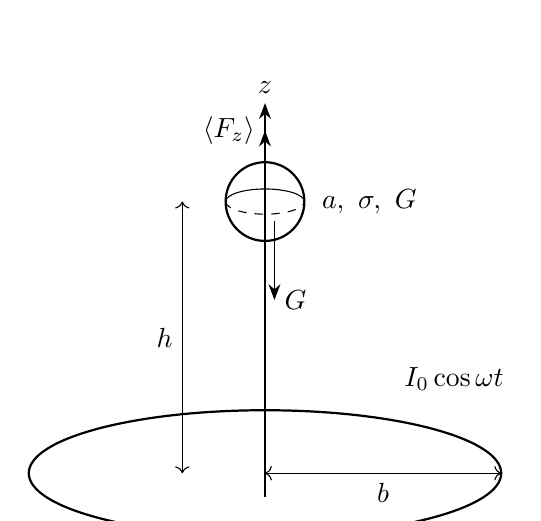
\begin{tikzpicture}[scale=1]
\draw[thick] (0,0) ellipse(3 and .8);
\draw[arr] (0,-.3)--(0,4.7) node[above] {$z$};
\draw[thick] (0,3.45) circle(.5);
\draw[dashed] (-.5,3.45) arc(180:360:.5 and .16);
\draw (-.5,3.45) arc(180:0:.5 and .16);
\node[right] at (.6,3.45) {$a,\ \sigma,\ G$};
\draw[<->] (-1.05,0)--(-1.05,3.45) node[midway,left] {$h$};
\draw[<->] (0,0)--(3,0) node[midway,below] {$b$};
\node at (2.4,1.2) {$I_0\cos\omega t$};
\draw[arr] (0,3.45)--(0,4.35) node[left] {$\langle F_z\rangle$};
\draw[arr] (.12,3.2)--(.12,2.2) node[right] {$G$};
\end{tikzpicture}
}
\ifdim\wd\diagrambox>.88\linewidth
\sbox{\diagrambox}{\resizebox{.88\linewidth}{!}{\usebox{\diagrambox}}}\fi
\ifdim\ht\diagrambox>.38\textheight
\resizebox{!}{.38\textheight}{\usebox{\diagrambox}}
\else\usebox{\diagrambox}\fi
\par\smallskip{\small 水平圆线圈与轴线上导体球\par}\endgroup\end{minipage}\end{center}

（1）将原来内部无磁场、半径为 \(a\)
的理想导体球（\(\sigma\to\infty\)）放在均匀稳恒外场
\(\boldsymbol B_e=B_e\hat{\boldsymbol z}\)
中。已知球外附加场等效于球心磁偶极矩 \(\boldsymbol m\) 的场

\[\boldsymbol B'=\frac{\mu_0}{4\pi r^3}
[3(\boldsymbol m\cdot\hat{\boldsymbol r})\hat{\boldsymbol r}-\boldsymbol m].\]

求 \(\boldsymbol m\) 和球面电流密度分布。

（2）求圆线圈在球心处的磁感应强度 \(\boldsymbol B(t)\)。

（3）求悬浮在给定高度 \(h\) 所需的电流幅值
\(I_0\)。假设频率足够高，球在悬浮位置附近的振动幅度可忽略。提示：磁偶极矩与外场均沿
\(z\) 轴时，安培力为 \(\boldsymbol F=m(dB_e/dz)\hat{\boldsymbol z}\)。

（4）把趋肤层内沿径向的涡电流近似为均匀分布，其余球内电流为零。求一个周期的平均热功率，最终式不含
\(\delta\)。

\clearpage

\section{第 7
题　大气温度、声速与远程声传播（40分）}\label{ux7b2c-7-ux9898-ux5927ux6c14ux6e29ux5ea6ux58f0ux901fux4e0eux8fdcux7a0bux58f0ux4f20ux64ad40ux5206}

大气最底部为对流层，厚度约10 km，温度随高度升高而降低；其上约10
km范围内温度近似不变，称同温层；更高的一段温度随高度升高而增加，称逆温层。

\begin{center}
\begin{minipage}{\linewidth}
\centering\begingroup\sbox{\diagrambox}{\small
\begin{tikzpicture}[scale=.92]
\fill[gray!20] (0,0) circle(1.6);
\draw (0,0) circle(1.6);
\draw (0,0) circle(2.1);
\draw (0,0) circle(2.6);
\draw (0,0) circle(3.1);
\node at (0,0) {地球};
\node[rotate=-45,font=\small] at (45:1.86) {对流层};
\node[rotate=-45,font=\small] at (45:2.36) {同温层};
\node[rotate=-45,font=\small] at (45:2.87) {逆温层};
\node at (0,-3.65) {层厚为示意，不按地球比例绘制};
\end{tikzpicture}
}
\ifdim\wd\diagrambox>.88\linewidth
\sbox{\diagrambox}{\resizebox{.88\linewidth}{!}{\usebox{\diagrambox}}}\fi
\ifdim\ht\diagrambox>.38\textheight
\resizebox{!}{.38\textheight}{\usebox{\diagrambox}}
\else\usebox{\diagrambox}\fi
\par\smallskip{\small 地球外围的三层简化大气\par}\endgroup\end{minipage}\end{center}

（1）把对流层的温度变化看成空气缓慢绝热上升的结果，求温度与高度 \(z\)
的关系。地表温度为 \(T_0\)，空气为理想气体，摩尔质量为 \(\mu\)，比热比
\(\gamma\) 为常数，普适气体常量为 \(R\)，重力加速度 \(g\) 视为常量。

（2）气体声速为 \(v_s=\sqrt{(dp/d\rho)_{\rm ad}}\)，\(p\)
为压强，\(\rho\)
为密度。不考虑风，求声速与温度的关系，讨论三层中声速随高度的变化。

（3）进一步简化：界面为平面；对流层与逆温层温度都为
\(-10^\circ\mathrm C\)，同温层为
\(-55^\circ\mathrm C\)。同温层内声源的声波入射至上下界面时，讨论不同入射角的折射与全反射，并画定性光路图。\(0^\circ\mathrm C=273.15\,\mathrm K\)。

（4）仍用各层恒温、两外层较暖的模型，但界面改为与地球同心的球面。声源和探测气球分别位于对流层或同温层。忽略地面反射和可发生折射时的反射，不考虑吸收。对四种位置组合，判断哪些能探测几千公里外的声音，哪些只能探测小于1000
km的声音，并估算解释。地球半径 \(R_e\simeq6371\,\mathrm{km}\)。

\clearpage

\section{第 8
题　X射线光谱与康普顿散射（40分）}\label{ux7b2c-8-ux9898-xux5c04ux7ebfux5149ux8c31ux4e0eux5eb7ux666eux987fux6563ux5c0440ux5206}

X射线光谱与光电子能谱可用于获取物质结构信息。X射线管由电子枪阴极和金属阳极组成；阴极电子被电压加速，与金属阳极碰撞后产生X射线，光谱包括连续轫致辐射和离散特征谱。选定波长的特征X射线照射材料靶，用X射线光谱仪与光电子能谱仪分别探测出射光子和电子。已知

\[R_\infty=10973731\,\mathrm{m^{-1}},\qquad
hc=1240\,\mathrm{nm\cdot eV}.\]

\begin{center}
\begin{minipage}{\linewidth}
\centering\begingroup\sbox{\diagrambox}{\small
\begin{tikzpicture}[scale=1]
\draw[rounded corners,thick] (-1,-.8) rectangle(.3,.8);
\node at (-.35,1.25) {X射线管};
\node at (-.35,-1.2) {电子轰击阳极};
\draw[arr,thick] (.3,0)--(3.5,0) node[midway,above] {入射光子};
\draw[thick] (3.5,-.65)--(3.5,.65);
\node at (3.5,-1.05) {材料靶};
\draw[arr] (3.5,0)--(6.3,-1.0) node[right] {X射线光谱仪};
\draw[arr] (3.5,0)--(5.5,1.35) node[right] {电子能谱仪};
\draw[dashed] (3.5,0)--(6.2,0);
\draw (4.3,0) arc(0:-19.65:.8);
\node at (4.65,-.26) {$\theta$};
\end{tikzpicture}
}
\ifdim\wd\diagrambox>.88\linewidth
\sbox{\diagrambox}{\resizebox{.88\linewidth}{!}{\usebox{\diagrambox}}}\fi
\ifdim\ht\diagrambox>.38\textheight
\resizebox{!}{.38\textheight}{\usebox{\diagrambox}}
\else\usebox{\diagrambox}\fi
\par\smallskip{\small X射线源、材料靶与两种探测器\par}\endgroup\end{minipage}\end{center}

（1）玻尔理论描述氢原子及类氢体系的能级。多电子原子的 \(n=1,2,3\)
壳层分别记为K、L、M。金属阳极原子的K壳层电子能量为
\(-20.1\,\mathrm{keV}\)。（i）电子至少需被多大电压加速，才可电离一个K壳层电子并使L壳层向K壳层跃迁发出K\(_\alpha\)特征X射线？（ii）该加速电压下连续X射线的最短波长是多少？前两项保留三位有效数字。（iii）已知K\(_\alpha\)光子能量为17.44
keV，计算该原子的核电荷数。

（2）波长为 \(\lambda_0\) 的K\(_\alpha\)光子与材料靶中初始静止、质量为
\(m\) 的电子散射。出射光子与入射光子的夹角为 \(\theta\)。求出射波长
\(\lambda_1\) 和电子动能。

（3）\(\theta=135^\circ\) 时，光谱有两个峰，分别位于 \(\lambda_0\)
与更长的 \(\lambda_1\)，后者较宽。说明两个峰的来源，以及 \(\lambda_1\)
峰较宽的原因。

\begin{center}
\begin{minipage}{\linewidth}
\centering\begingroup\sbox{\diagrambox}{\small
\begin{tikzpicture}[xscale=1.05,yscale=1]
\draw[arr] (0,0)--(7.4,0) node[right] {$\lambda$};
\draw[arr] (0,0)--(0,3.4) node[above] {相对谱强度};
\draw[thick,domain=.2:7,samples=140]
plot(\x,{.2+2.25*exp(-(\x-2)*(\x-2)/.06)+2.7*exp(-(\x-5)*(\x-5)/.45)});
\draw[dashed] (2,0)--(2,2.5); \draw[dashed] (5,0)--(5,3);
\node[below] at (2,0) {$\lambda_0$}; \node[below] at (5,0) {$\lambda_1$};
\node at (2,3.0) {近弹性峰}; \node at (5,3.5) {康普顿峰};
\node at (3.5,-.9) {峰位与峰宽的定性示意，不作定量读数};
\end{tikzpicture}
}
\ifdim\wd\diagrambox>.88\linewidth
\sbox{\diagrambox}{\resizebox{.88\linewidth}{!}{\usebox{\diagrambox}}}\fi
\ifdim\ht\diagrambox>.38\textheight
\resizebox{!}{.38\textheight}{\usebox{\diagrambox}}
\else\usebox{\diagrambox}\fi
\par\smallskip{\small 原题双峰关系的定性重绘：移位峰较宽\par}\endgroup\end{minipage}\end{center}

\end{document}
